\documentclass{article}

\usepackage{arxiv}

\usepackage[utf8]{inputenc} % allow utf-8 input
\usepackage[T1]{fontenc}    % use 8-bit T1 fonts
\usepackage{hyperref}       % hyperlinks
\usepackage{url}            % simple URL typesetting
\usepackage{booktabs}       % professional-quality tables
\usepackage{amsfonts}       % blackboard math symbols
\usepackage{nicefrac}       % compact symbols for 1/2, etc.
\usepackage{microtype}      % microtypography
\usepackage{lipsum}
\usepackage{graphicx}
\usepackage[
    backend=biber,
    style=numeric,
  ]{biblatex}
\bibliography{references}
\title{Nested 3D neural networks for kidney and tumor segmentation}


\author{
  Olmo Zavala-Romero,\\
  %\thanks{Use footnote for providing further webpage, alternative address)---\emph{not} for acknowledging funding agencies.} \\
  Department of Radiation Oncology\\
  Sylvester Comprehensive Cancer Center, University of Miami\\
  1475 NW 12th Avenue Miami, FL 33136\\
  \texttt{osz1@miami.edu} \\
  %% examples of more authors
  \And
  Javier \\
  \texttt{} \\
  \AND
  Ignacio Alvarez Illan,\\
  Signal Theory and Communications Department\\
  Universidad de Granada, 18071 Granada, Spain\\
  \texttt{illan@ugr.es} \\
  \AND
  Radka Stoyanova\\
  Department of Radiation Oncology\\
  Sylvester Comprehensive Cancer Center, University of Miami\\
  1475 NW 12th Avenue Miami, FL 33136\\
  \texttt{rstoyanova@med.miami.edu} \\
  \AND
 Adrian L. Breto\\
 Department of Radiation Oncology\\
 Sylvester Comprehensive Cancer Center, University of Miami\\
 1475 NW 12th Avenue
 Miami, FL 33136\\
 \texttt{a.breto@umiami.edu} \\
  \AND
Isaac
 \AND
  Jorge Zavala-Hidalgo\\
  Centro de Ciencias de la Atm\'osfera\\
  Universidad Nacional Aut\'onoma de M\'exico, Mexico City, M'exico\\
  \texttt{jzavala@atmosfera.unam.mx} \\
  \AND
  Rosario Romero-Centeno\\
  Centro de Ciencias de la Atm\'osfera\\
  Universidad Nacional Aut\'onoma de M\'exico, Mexico City, M\'exico\\
  \texttt{rosario@atmosfera.unam.mx} \\
}

\begin{document}
\maketitle

\begin{abstract}

\end{abstract}


% keywords can be removed
\keywords{First keyword \and Second keyword \and More}

\section{Introduction}
\label{sec:intro}

Kidney cancer has an high number of diagnosed cases each year, being invasive techniques the most common treatment\cite{sun_treatment_2012}. Machine learning techniques have been proven to provide valuable tools in medical imaging, increasing the accuracy in diagnosis for several diseases\cite{erickson_machine_2017}. In recent years, deep learning techniques have increased the performance of classical machine learning approaches in several imaging problems, including medical image analysis\cite{litjens_survey_2017}. In this work, we propose a deep learning approach for kidney cancer detection and segmentation, as participants of the Kits19 challenge.


The code will be freely available for others to use on their own data at \url{https://github.com/naclet/Kits19} after
the publication of this work. 

\section{Methodology}
\label{sec:methods}

\subsection{Data}
\label{sec:data}

The data used in this study belongs to the Kits19 challenge\cite{heller_kits19_2019}, which consists of 544 patients who underwent radical nephrectomy of partial nephrectomy, reviewed at the University of Minnesota, with a selection of 300 patients that met the inclusion criteria. These patients have annotated CT abdominal images, with two annotations: kidneys and tumors. The data was separated in training and testing data, and the annotations where only available in the 210 patients training set to the challenge participants. 

\subsection{Preprocessing}
\label{sec:prepro}
The proposed network architecture, described in section \ref{sec:nnarc}, receives and image of size $168^3$. In order to
obtain an image with this dimensions for all our training cases, they had to be preprocessed to a region of interest (ROI) with
these dimensions.  The proprocessing steps include: a resampling of the image to an isotropic pixel size of $2 \times 2 \times 2$ mm and cropping the CT image to a resolution of $168^3$ from the center of the image, if the CT image was smaller, the ROI is padded
with zeros. Finallly the ROI is normalized so that the intensity values of all the images range from 0 to 1. 

\subsection{Neural Network Architecture}
\label{sec:nnarc}
The proposed deep learning architecture is 3D V-Net [REF] with fourteen convolutional layers. This network is
first trained to learn how to segment the kidneys, after that the weights are saved and 
the same architecture its used to learn how to segment the tumors. The architecture of this 
network is shown in figure \ref{fig:arc}.  Each convolutional layer has relu as the activation function and
filters size $3\times 3 \times 3$, with the exception of the last convolutional layer which 
uses a sigmoid activation function. Each convolutional layer in the decoding phase has batch normalization to improve the generalization of the network. Finally, the dimensions of the input and output images is $168^3$. 

The training dataset is randomly splitted into $90\%$ for training and $10\%$ for validation.  
The network uses stochastic gradient descent as the optimization method, the number of steps per epoch is
100 and the number of steps when computing the metrics on the validation set is 20. The trainig is
stopped after 1000 iterations or when the loss function on the validation set do not improves after
90 iterations. 

The difference between training the network to learn how to segment kidneys vs tumors, lays on the 
loss function being used. In both cases, the metric that is minimized is the negative Sorensen-Dice coefficient (DSC) \ref{eq:dsc}
\cite{dice1945measures}.  But, in the case of the training for tumors, the DSC only takes into account the pixels that are
inside the kidneys. This helps the network to avoid learning only zero-valued weights. 

\begin{equation}
    loss = - \frac{2 \sum_{i=1}^{N}p_it_i}{\sum_{i=1}^{N}p_i + \sum_{i=1}^{N}t_i + \varepsilon}
    \label{eq:dsc}
\end{equation}

\begin{figure}[h]
    \centering
    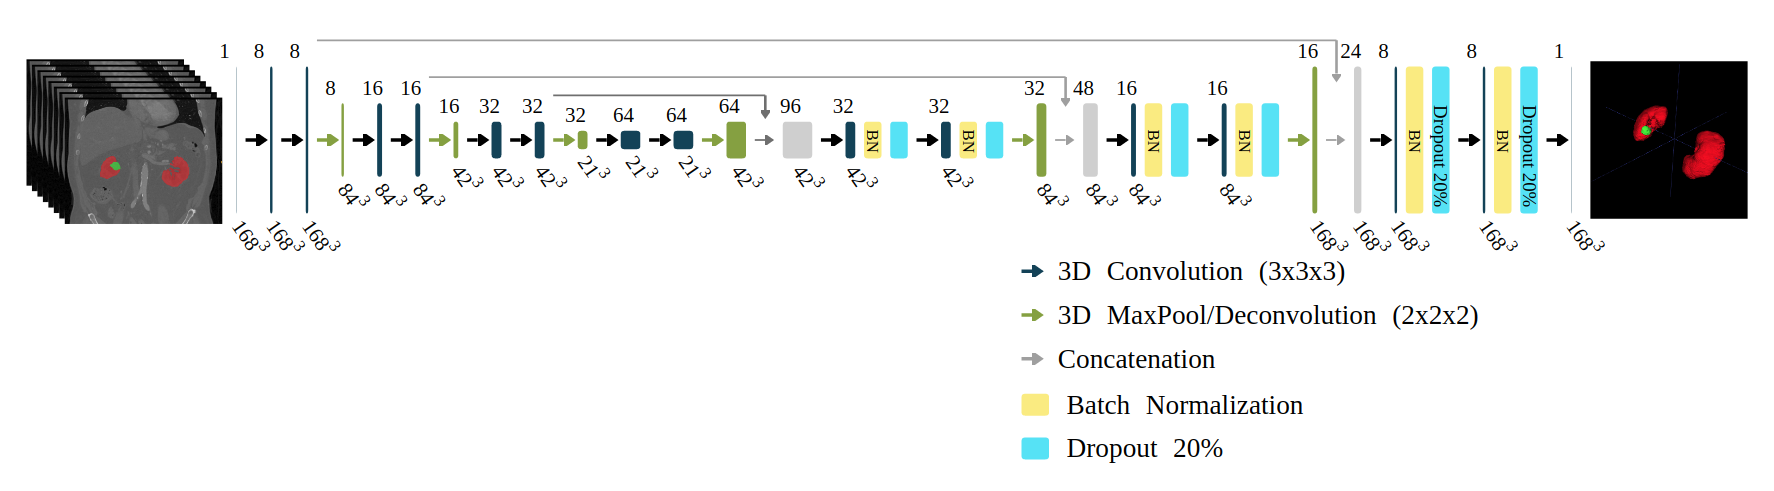
\includegraphics[totalheight=.18\textheight]{imgs/nn.png}
    \caption{NN architecture }
    \label{fig:arc}
\end{figure}


\subsection{Posprocessing}
\label{sec:post}
For the final classifications, the network is used with the trained weights to predict the locations of the kidneys. During this process the CT image gets preproccessed (resampled, cropped and normalized) and the prediction is made on the obtained ROI.
After that, only the top three structures  larger than 10 cubic centimeters are kept (if available). Then, the tumors
are segmented using the same network but the proper weights for predicting for tumors. The resulting output is masked
by the predicted kidneys in the previous step. Finally both segmentaitons are interpolated into its original CT resolution using Nearest Neighbor implementation in Simple ITK. 

\section{Conslusions}
\label{sec:conlusions}
SUMMARY here

The segmentation of the kidneys can be improved if the network used for training has a larger resolution than $168^3$
and the resampled ROI has a smaller pixel size than $2 \times 2 \times 2$ mm. The main reason why this was not tested
is the restriction we had in our computer resourcers, for this work four NVIDIA GeForce GTX 1080 were used for the trainnig.
These GPUs have 8 GB of memory, and when testing larger models we ran out of memory. 

\printbibliography

\end{document}
